\subsubsection{Modification}

The modify flow are similar as \textit{INTEGER} type, remove the key which don't needed and add the count if the byte is the same. So follow the example in figure \ref{fig:algorithm:real:insertion:example} and then modify -$0.01$ to +$0.0$ (because zero don't contain positive or negative sign, so using positive sign should be fine), the table will look like figure \ref{fig:algorithm:real:modification:example} and the time complexity be $O(b)$.

\begin{figure}[h]
\centering
%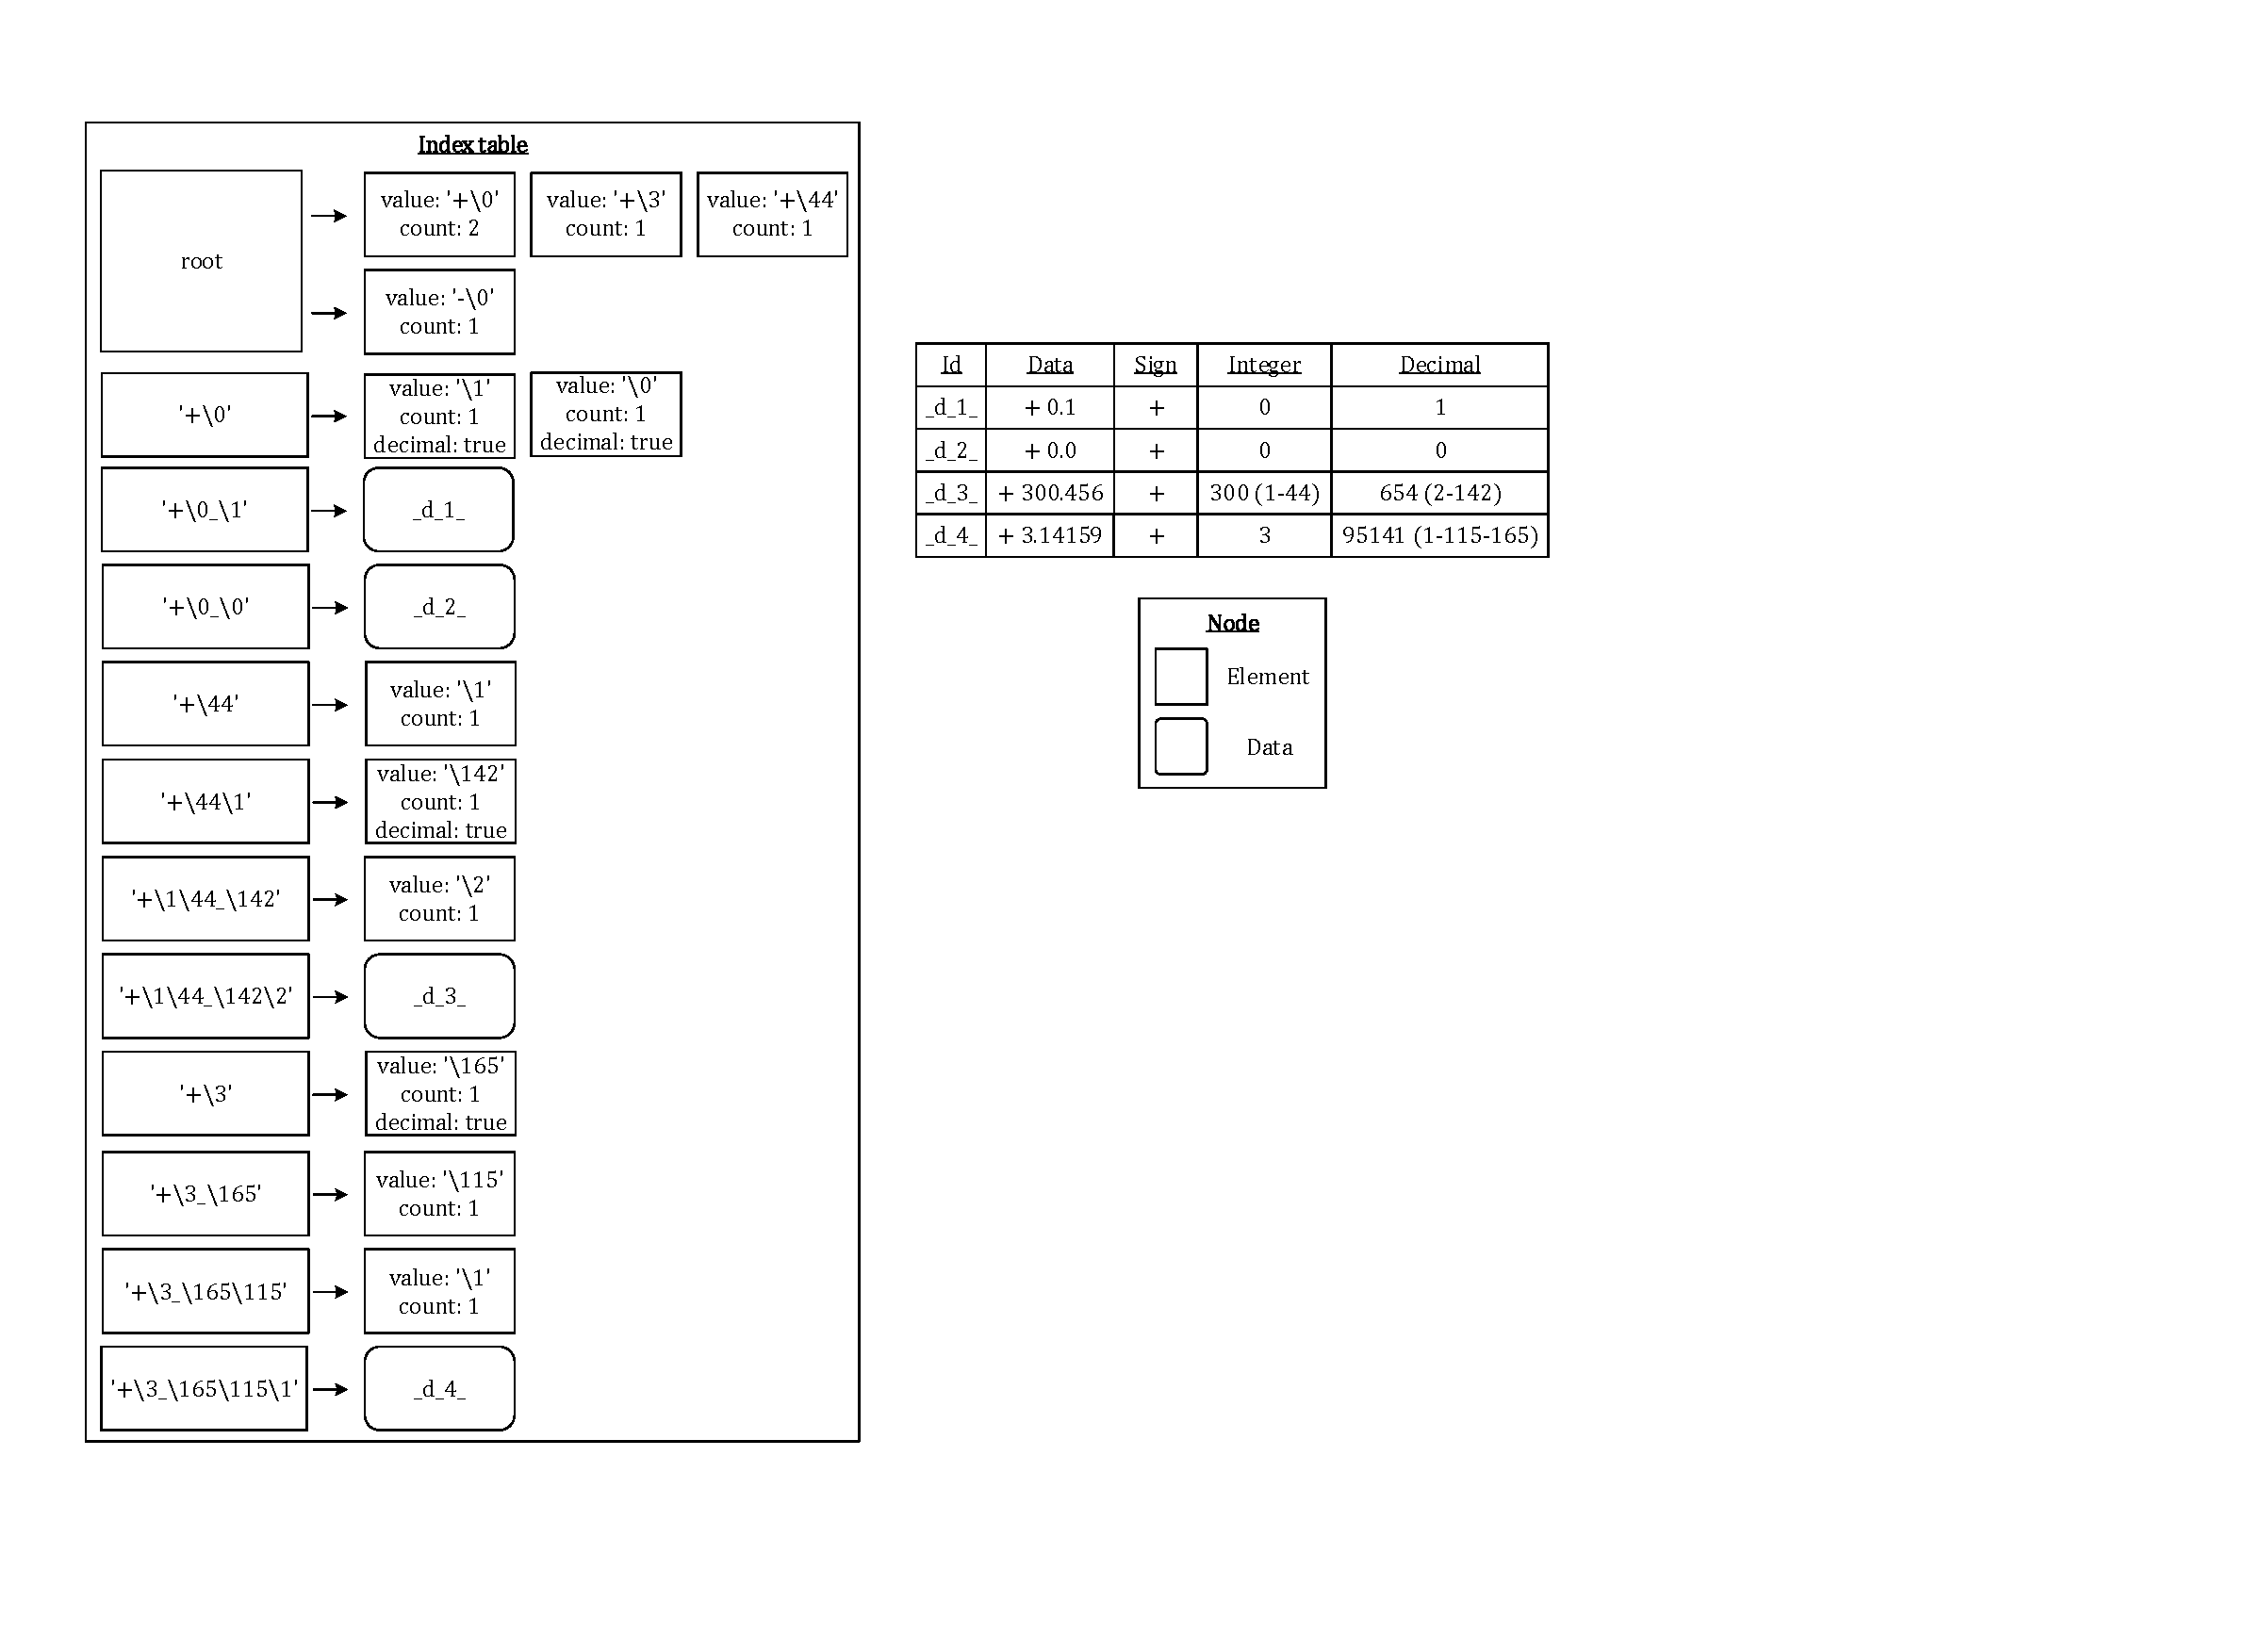
\includegraphics[scale=0.5]{./algorithm/real/pic/modification/example_v4.pdf}
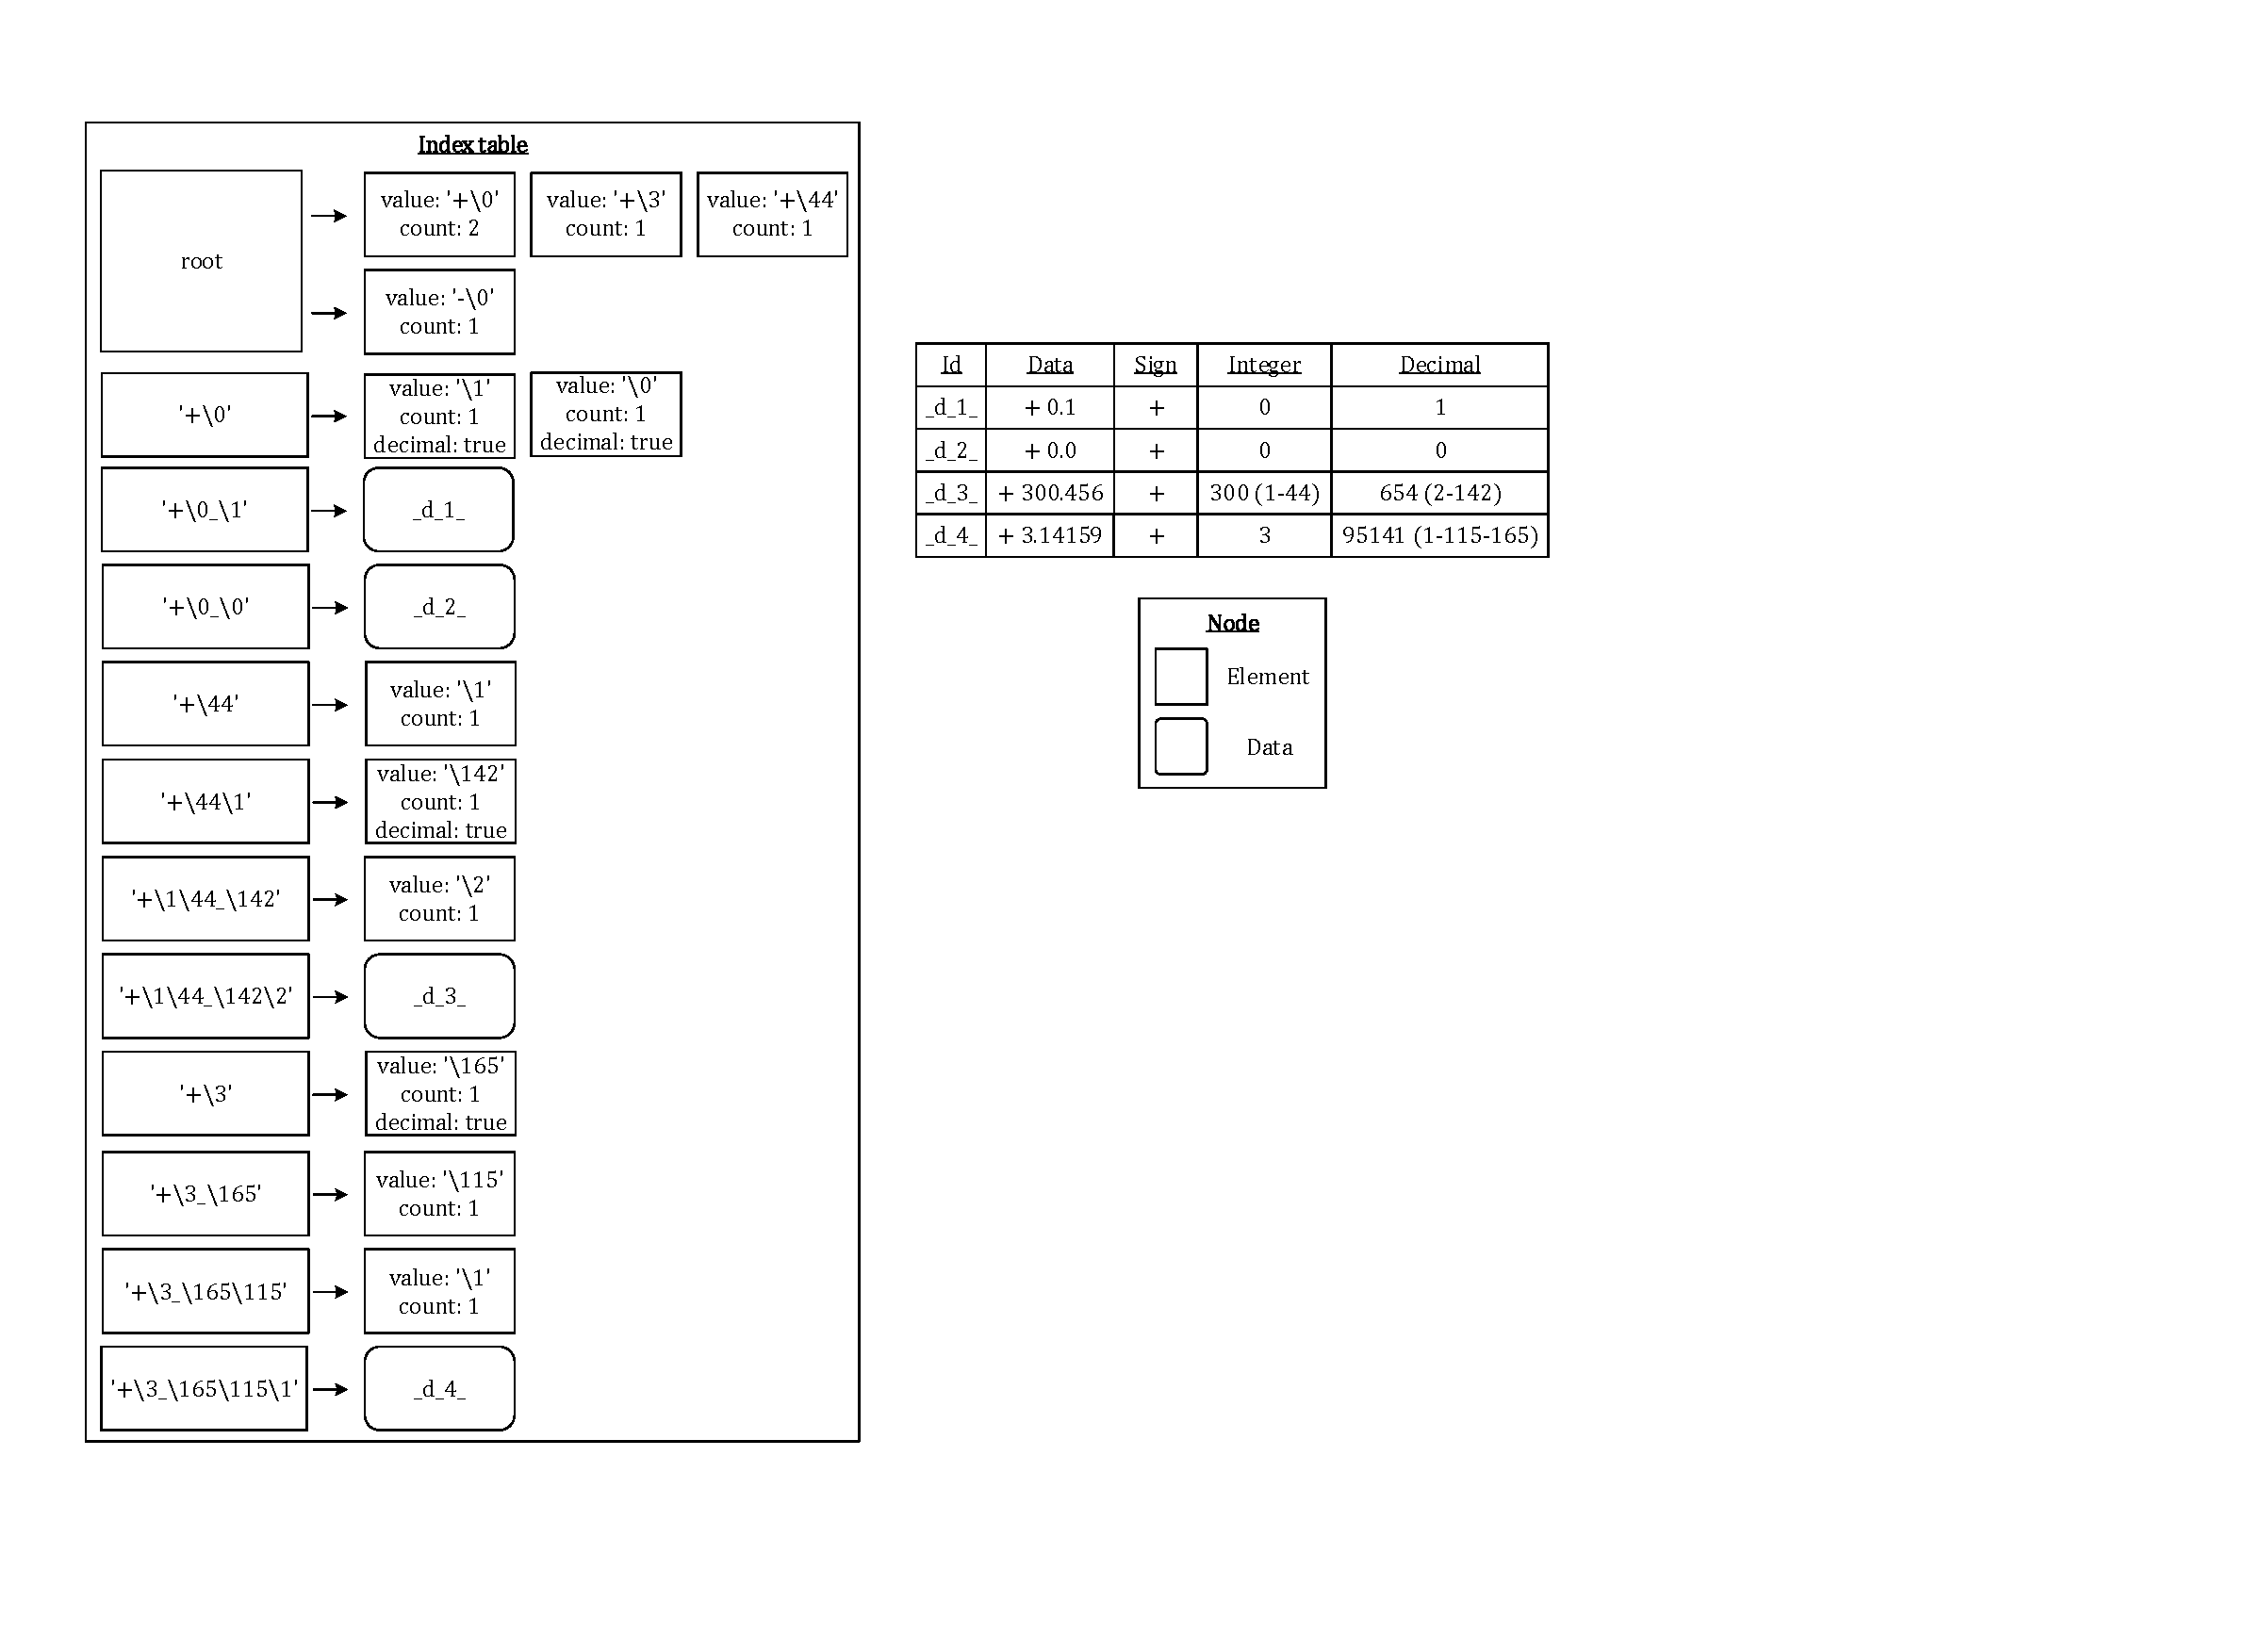
\includegraphics[width=0.8\textwidth]{./algorithm/real/pic/modification/example_v4.pdf}
\caption{The table after modified the value.}
\label{fig:algorithm:real:modification:example}
\end{figure}

